\documentclass{article}
% \usepackage{fullpage}

\usepackage{template}

\usepackage{tikz}
\usetikzlibrary{positioning,fit,calc}

\header{%
  assignment={\texttt{mininet} Guide},%
  course={IN[59]570: Distributed Objects},%
  authors={Oleks Shturmov \texttt{<\href{mailto:oleks@oleks.info}{oleks@oleks.info}>}},%
  affiliation={Department of Informatics\\University of Oslo},%
  shortAffiliation={IFI/UiO},%
  date={\today}%
}

\newcommand{\mininet}{\texttt{mininet}}

\begin{document}

\maketitle

\mininet{} is a tool for light-weight computer network emulation. To
this end it uses operating-system (OS) level virtualisation, similar
to ``container'' technologies like Docker. \mininet{} allows us to
test that our distributed software behaves as expected in various
concrete computer networking scenarios.

This is a short guide to using \mininet{} in the Distributed Objects
(IN[59]570) course at UiO. Section \ref{sec:mininet} covers our
recommended way to install \mininet{}, while section \ref{sec:emerald}
focuses on running Emerald code on top of that installation.

\section{Installing \mininet{}}

\label{sec:mininet}

You can either install \mininet{} natively; or run it in a VM, or a
container. We recommend one of the latter options since \mininet{},
rather unfortunately, \textbf{requires root priveleges for network
emulation}. That said, there is no need to expose your personal
machine, or network, to \mininet{}. Using a container or a VM allows
you to hand \mininet{} its desired privileges, but only to a confined,
simulated machine. Figure \ref{fig:mininet-basics} illustrates the
setup we will create.

\begin{figure}[htbp!]
\centering

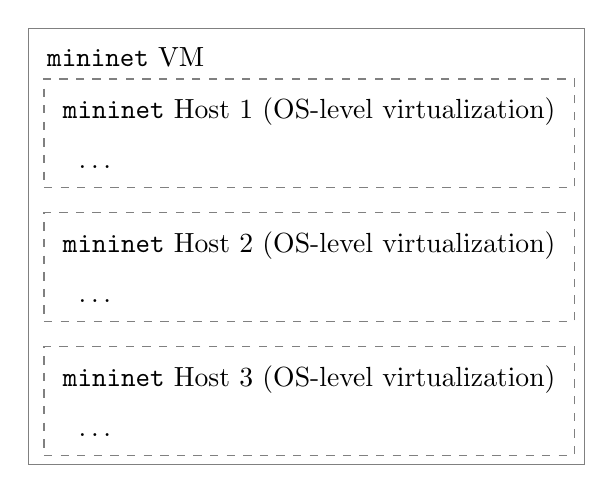
\begin{tikzpicture}[
  node distance=7mm,
  title/.style={},
  subtitle/.style={anchor=west},
  typetag/.style={anchor=west}
]
  \node (vm) [title] { \texttt{mininet} VM };

  \node (h1) [below=of vm.west, subtitle, xshift=2mm] { \texttt{mininet} Host 1 (OS-level virtualization) };
  \node (d1) [below=of h1.west, typetag, xshift=2mm] { \ldots };

  \node (h1wrap) [draw=black!50, fit={(h1) (d1)}, dashed] {};

  \node (h2) [below=of h1.west, subtitle, yshift=-10mm] { \texttt{mininet} Host 2 (OS-level virtualization) };
  \node (d2) [below=of h2.west, typetag, xshift=2mm] { \ldots };

  \node (h2wrap) [draw=black!50, fit={(h2) (d2)}, dashed] {};

  \node (h3) [below=of h2.west, subtitle, yshift=-10mm] { \texttt{mininet} Host 3 (OS-level virtualization) };
  \node (d3) [below=of h3.west, typetag, xshift=2mm] { \ldots };

  \node (h3wrap) [draw=black!50, fit={(h3) (d3)}, dashed] {};

  \node [draw=black!50, fit={(vm) (h1wrap) (h2wrap) (h3wrap)}] {};

\end{tikzpicture}


\caption{Illustration of a \mininet{} setup; with \mininet{} running
in the official \mininet{} VM, emulating 3 hosts. We use a solid line
to indicate a solid virtualization boundary, and dashed lines for a
softer, OS-level one. }

\label{fig:mininet-basics}

\end{figure}

Not only does running \mininet{} in a dedicated VM provide for a solid
boundary between our experiments and your personal machine, it is also
the recommended way to get started according to the official
documentation:

\begin{center}

\url{https://mininet.org/download/\#option-1-mininet-vm-installation-easy-recommended}

\end{center}

After you download and setup the VM with your favourite virtualisation
technology (e.g., VirtualBox, VMware Fusion, QEMU); we can recommend
to setup SSH port-forwarding, and connect to the VM via SSH. This is
done by configuring the VM in your virtualisation software.

\textbf{We will assume that you set host port 8022 to be forwarded to
port 22 (SSH port) inside the VM}. However, if your port 8022 is taken
by some other software, feel free to use another port.

\textbf{The username is \texttt{mininet}, so is the password}, and
password-based login via SSH is enabled by default. Here, we have no need
to harden this boundary.

If everything is setup correctly, you should be able to do the
following in your favourite command-line shell:

\begin{lstlisting}
$ ssh -p 8022 mininet@localhost
mininet@localhost's password: mininet
Welcome to Ubuntu 20.04.6 LTS (GNU/Linux 5.4.0-205-generic x86_64)

 * Documentation:  https://help.ubuntu.com
 * Management:     https://landscape.canonical.com
 * Support:        https://ubuntu.com/pro
New release '22.04.5 LTS' available.
Run 'do-release-upgrade' to upgrade to it.

Last login: Wed Feb 19 02:30:13 2025 from 10.0.2.2
mininet@mininet-vm:~$
\end{lstlisting}

We will now copy some files over to the VM, which will make it easier
to startup a \mininet{} instance as illustrated in Figure \ref{fig:mininet-basics}.

First, download the files \texttt{config.py} and \texttt{launch.sh}
from the following address to your local machine:

\begin{center}
\url{https://github.com/emerald/in5570v25/tree/main/mininet}
\end{center}

Now, copy them to the VM (NB! With \texttt{scp} (unlike \texttt{ssh}),
the port is specified with \texttt{-P} instead of \texttt{-p}):

\begin{lstlisting}
$ scp -P 8022 launch.sh config.py mininet@localhost:/home/mininet/in5570v25/
mininet@localhost's password: mininet
launch.sh                            100%  376   207.2KB/s   00:00
config.py                            100%  931     1.4MB/s   00:00
\end{lstlisting}

Now, inside the VM, run the \texttt{launch.sh} script, which will
create a network according to the configuration \texttt{config.py}:

\begin{lstlisting}
mininet@mininet-vm:~$ ./launch.sh
*** Creating network
*** Adding controller
*** Adding hosts:
h1 h2 h3 nat0
*** Adding switches:
s1 s2
*** Adding links:
(h1, s1) (s1, nat0) (s1, s2) (s2, h2) (s2, h3)
*** Configuring hosts
h1 h2 h3 nat0
Error starting terms: Cannot connect to display
*** Starting controller
c0
*** Starting 2 switches
s1 s2 ...
*** Starting CLI:
mininet>
\end{lstlisting}

At this point, we now have a setup as in Figure
\ref{fig:mininet-basics}, with the hosts named \texttt{h1},
\texttt{h2}, and \texttt{h3}, respectively. We can interact with these
hosts from the \mininet{} shell. For instance, to see that each host
has a unique IP address:

\begin{lstlisting}
mininet> h1 hostname -I
10.0.0.1
mininet> h2 hostname -I
10.0.0.2
mininet> h3 hostname -I
10.0.0.3
\end{lstlisting}

Type \texttt{exit} to shutdown the \mininet{} emulation and go back to
the regular VM shell. Remember that you can also start another SSH
session with the VM, and keep the \mininet{} network alive. 

\section{Running Emerald}

\label{sec:emerald}

Unfortunately, but also expectedly, the \mininet{} VM is ill-braced for Emerald.

One way to circumvent this is to leverage the fact that we already
have a Docker image inside of which Emerald can run. Hence, we will go
for a setup as illustrated in Figure \ref{fig:mininet-docker}. It may
seem silly to do nested OS-level virtualisation; but the mechanism, in
general, is designed to be compositional in this manner.

\begin{figure}[htbp!]
\centering
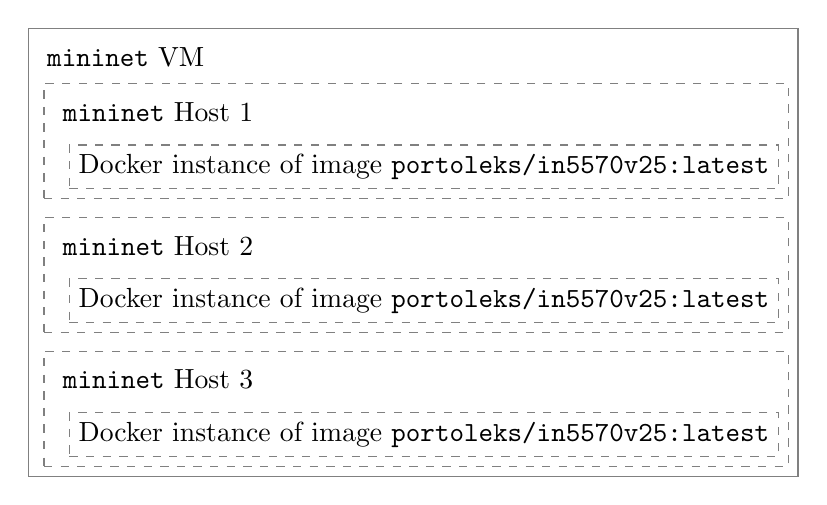
\begin{tikzpicture}[
  node distance=7mm,
  title/.style={},
  subtitle/.style={anchor=west},
  typetag/.style={draw=black!50, dashed, anchor=west}
]
  \node (vm) [title] { \texttt{mininet} VM };

  \node (h1) [below=of vm.west, subtitle, xshift=2mm] { \texttt{mininet} Host 1 };
  \node (d1) [below=of h1.west, typetag, xshift=2mm] { Docker instance of image \texttt{portoleks/in5570v25:latest} };

  \node (h1wrap) [draw=black!50, fit={(h1) (d1)}, dashed] {};

  \node (h2) [below=of h1.west, subtitle, yshift=-10mm] { \texttt{mininet} Host 2 };
  \node (d2) [below=of h2.west, typetag, xshift=2mm] { Docker instance of image \texttt{portoleks/in5570v25:latest} };

  \node (h2wrap) [draw=black!50, fit={(h2) (d2)}, dashed] {};

  \node (h3) [below=of h2.west, subtitle, yshift=-10mm] { \texttt{mininet} Host 3 };
  \node (d3) [below=of h3.west, typetag, xshift=2mm] { Docker instance of image \texttt{portoleks/in5570v25:latest} };

  \node (h3wrap) [draw=black!50, fit={(h3) (d3)}, dashed] {};

  \node [draw=black!50, fit={(vm) (h1wrap) (h2wrap) (h3wrap)}] {};

\end{tikzpicture}


\caption{Illustration of a \mininet{} setup; with \mininet{} running
in the official \mininet{} VM, emulating 3 hosts. We use a solid line
to indicate a solid virtualization boundary, and dashed lines for a
softer, OS-level one. }

\label{fig:mininet-docker}

\end{figure}

First, go ahead and install \texttt{docker.io} package inside the VM:

\begin{lstlisting}
mininet@mininet-vm:~$ sudo apt-get update
mininet@mininet-vm:~$ sudo apt-get upgrade
mininet@mininet-vm:~$ sudo apt-get install docker.io
\end{lstlisting}

Download the files \texttt{in\_docker.sh}
from the following address to your local machine:

\begin{center}
\url{https://github.com/emerald/in5570v25/tree/main/mininet}
\end{center}

Copy it to the VM:

\begin{lstlisting}
$ scp -P 8022 in_docker.sh mininet@localhost:/home/mininet/in5570v25/
mininet@localhost's password: mininet
in_docker.sh                         100%  376   207.2KB/s   00:00
\end{lstlisting}

\end{document}
